% https://github.com/SaverioMonaco/UniPD-Thesis-Template

\documentclass[BSc,italian]{unipdthesis}
\usepackage{lipsum}
\usepackage[Lenny]{fncychap}

% Add here all your information:
% Inserisci qui tutte le informazioni richieste:

% MSc, BSc, VO, PHD...
\def\thesistype{BSc}

% Name of the c
\def\coursename{Physics of Data}

% Who's writing this
% L'autore
\def\thesisauthor{Albert Einstein}

% Title of the thesis
% Titolo della tesi
\def\thesistitle{The equation of everything}

% Academic Year
% Anno accademico
\def\year{2021-2022}

% Dimension of the departement logo (in \linewith)
% Dimensione dell'immagine del dipartimento
\def\logocoursedim{.8}
\def\logocourse{./imgs/dfa_logo}

\begin{document}
\author{\thesisauthor}
\title{\thesistitle}
\aayear{\year}

\begin{supervisors}
   \supervisor{Chiar.mo}{Prof.}{A. Nyone}
   \supervisor{}{Dr.}{S. One Else}
\end{supervisors}

\maketitlepage

\tableofcontents

\chapter*{\iflanguage{italian}{Introduzione}{Introduction}}
\addcontentsline{toc}{chapter}{\iflanguage{italian}{Introduzione}{Introduction}}

\lipsum[20]

\chapter{\iflanguage{italian}{Stato dell'arte}{State of the art}}

\section{\iflanguage{italian}{Titolo della sezione}{Section title}}

\subsection{\iflanguage{italian}{Titolo del paragrafo}{Subsection title}}

\lipsum[20] \cite{Resnick:03} \lipsum[5]

\lipsum[40]
Inline equation $\nabla\cdot{\bf B} = 0$.
\lipsum[20]

\begin{figure}[t]
\centering
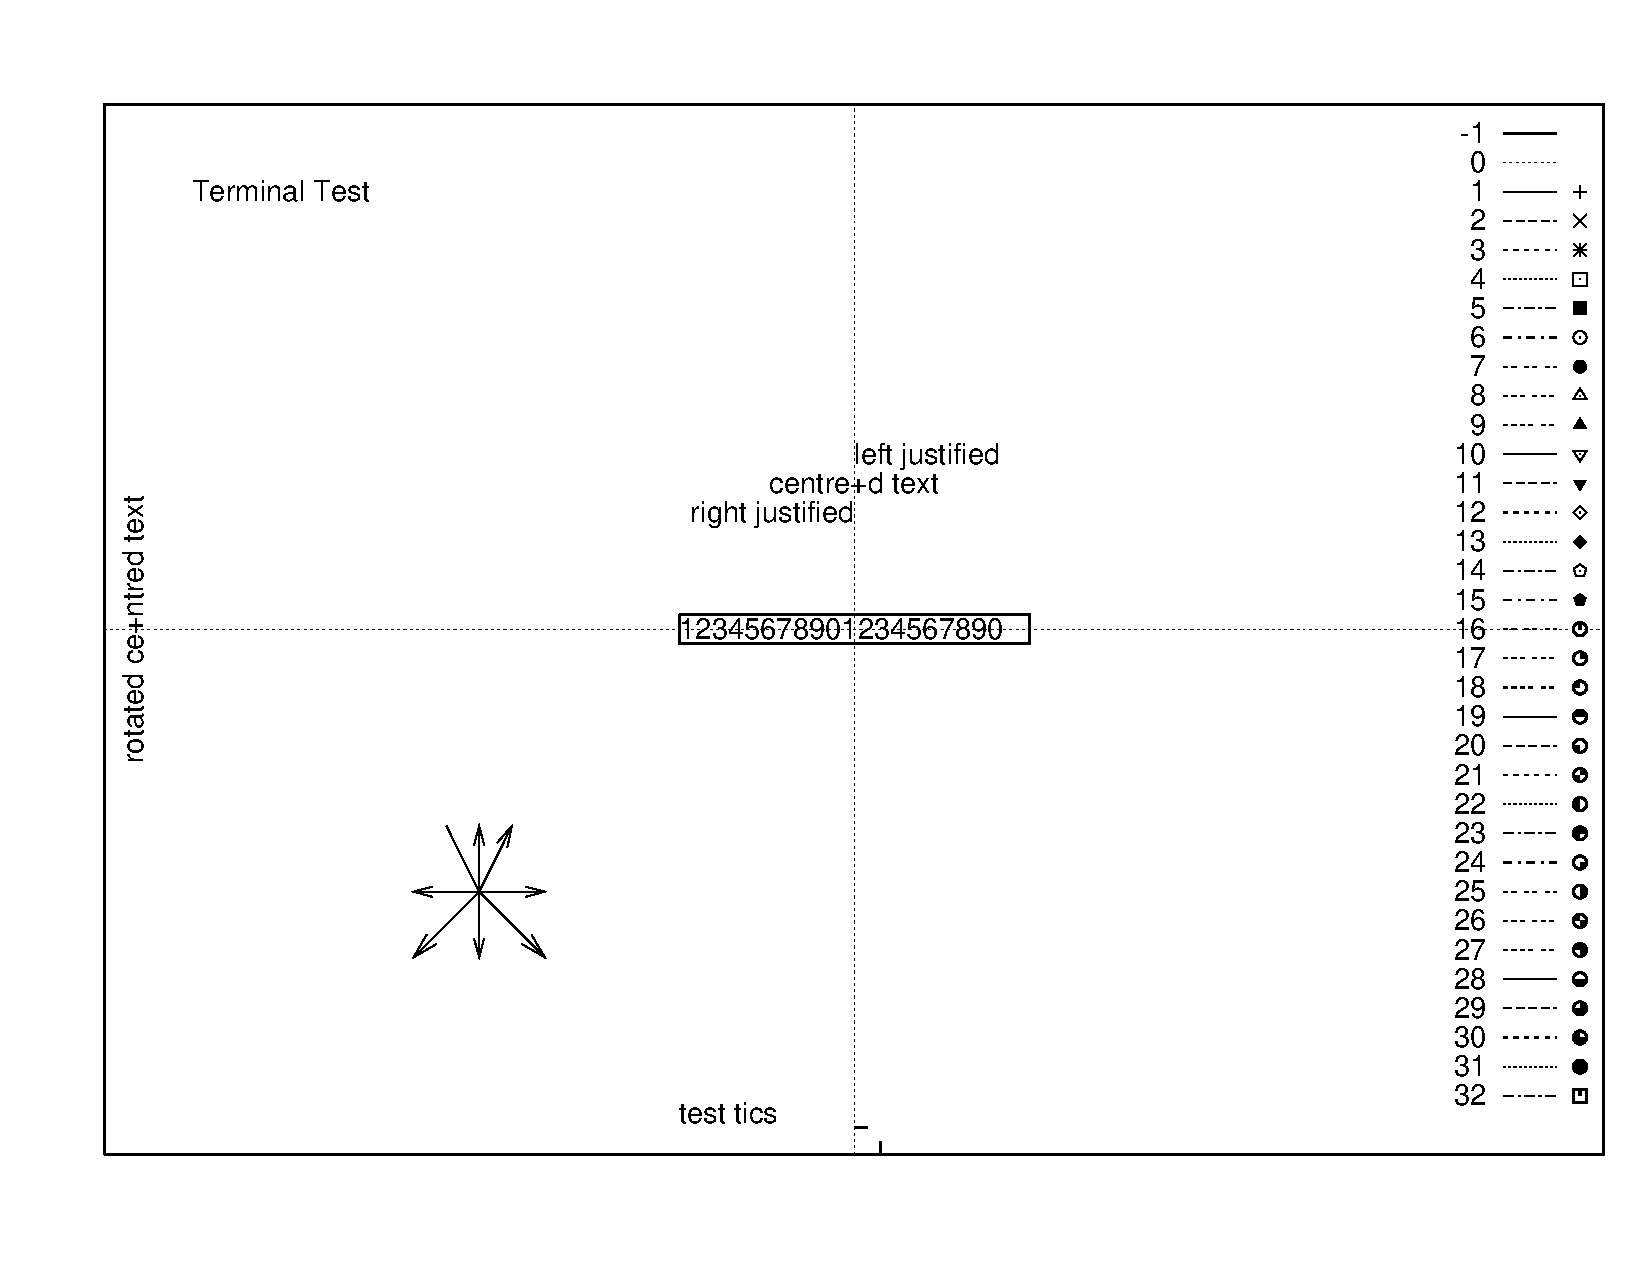
\includegraphics[width=0.8\columnwidth]{esempio.pdf}
\caption{Caption}
\label{fig:esempio}
\end{figure}

Cf.\ Fig.~\ref{fig:esempio}.
\lipsum[30]
\begin{equation}
f(z) = \oint \frac{f(\zeta)}{\zeta - z} d\zeta .
\end{equation}
\lipsum[10]

\chapter*{\iflanguage{italian}{Conclusioni}{Conclusions}}
\addcontentsline{toc}{chapter}{\iflanguage{italian}{Conclusioni}{Conclusions}}

\lipsum[20]

\addcontentsline{toc}{chapter}{\iflanguage{italian}{Bibliografia}{Bibliography}}
\bibliographystyle{mprsty}
\bibliography{biblio}

\chapter*{\iflanguage{italian}{Ringraziamenti}{Acknowledgements}}
\addcontentsline{toc}{chapter}{\iflanguage{italian}{Ringraziamenti}{Acknowledgements}}

\lipsum[20]

\end{document}
